本章作为开篇，旨在说明软件架构在软件开发中扮演的角色。它将聚焦于设计 C++ 解决方案架构时需要牢记的关键方面。我们将讨论如何设计出高效、且具有便捷而实用接口的代码。我们还会展示领域驱动方法如何与敏捷原则相辅相成，并同时指导代码与架构。

本章将涵盖以下主题：

\begin{itemize}
\item 理解软件架构
\item 恰当架构的重要性
\item 优秀架构的基本要素
\item 运用敏捷原则开发架构
\item C++ 的哲学
\item 遵循 SOLID 与 DRY 原则
\item 耦合与内聚
\end{itemize}

\section{如何充分利用本书——了解你的免费福利}

解锁随购买附赠的专属\textbf{免费}福利，这些福利经过精心设计，能为你的学习之旅加速，助你无拘无束地学习。

下面是本书附赠内容的快速概览：

\subsection{新一代阅读器}

\begin{center}
\begin{tabularx}{\textwidth}{XX}
\toprule
\begin{center}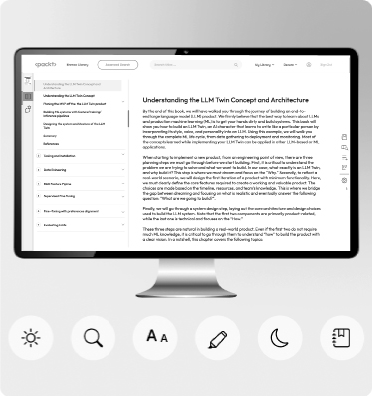
\includegraphics[width=0.450\linewidth]{images/nextgen.png}\end{center} {\fontsize{8bp}{10.5bp}\selectfont 图 1.1：新一代 Packt Reader 功能示意图\par} & 我们的网页版阅读器旨在帮助你高效学习，具备以下功能： \begin{itemize} \item \textbf{ 多设备进度同步}：随时随地学习，进度无缝同步。 \item \textbf{ 高亮与笔记}：把阅读转化为持久的知识。 \item \textbf{ 书签}：随时重温最重要的学习内容。 \item \textbf{ 深色模式}：切换到深色或棕褐模式，专注阅读，减轻眼疲劳。 \end{itemize} \\
\midrule
\bottomrule
\end{tabularx}
\end{center}

\subsection{交互式 AI 助手（beta）}

\begin{center}
\begin{tabularx}{\textwidth}{XX}
\toprule
\begin{center}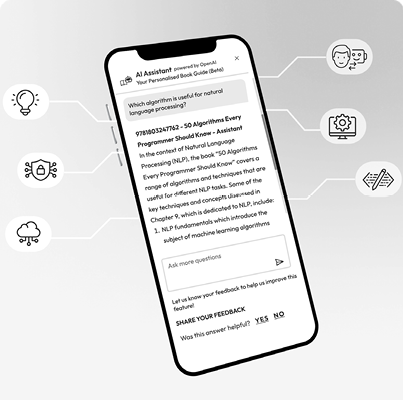
\includegraphics[width=0.450\linewidth]{images/InteractiveAIAssistantgrayscaled.png}\end{center} {\fontsize{8bp}{10.5bp}\selectfont 图 1.2：Packt 的 AI 助手示意图\par} & 我们的交互式 AI 助手基于本书内容训练而成，旨在最大化你的学习体验。它具备以下功能： \begin{itemize} \item \textbf{ 一键总结}：总结关键章节或整章内容。 \item \textbf{ AI 代码讲解}：在下一代 Packt Reader 中，点击每个代码块上方的 \textbf{Explain} 按钮，即可获得由 AI 驱动的代码讲解。 \end{itemize} \emph{注意：AI 助手是下一代 Packt Reader 的一部分，目前仍处于 beta 阶段。 } \\
\midrule
\bottomrule
\end{tabularx}
\end{center}

\subsection{无 DRM 的 PDF 或 ePub 版本}

\begin{center}
\begin{tabularx}{\textwidth}{XX}
\toprule
\begin{center}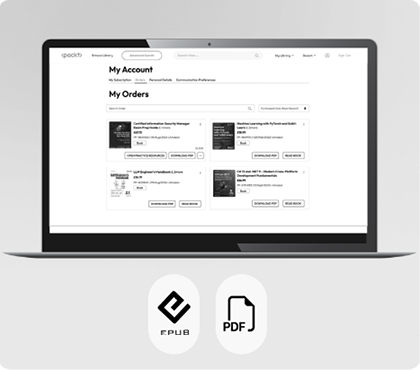
\includegraphics[width=0.467\linewidth]{images/freepdfandepub.png}\end{center} {\fontsize{8bp}{10.5bp}\selectfont 图 1.3：免费的 PDF 与 ePub\par} & 购买本书即可享受以下权益，让你的学习不受限制： \begin{itemize} \item 借助本书无 DRM 的 PDF 副本，随时随地学习。 \item 用你喜欢的电子阅读器阅读本书无 DRM 的 ePub 版本进行学习。 \end{itemize} \\
\midrule
\bottomrule
\end{tabularx}
\end{center}

\begin{center}
\begin{tabularx}{\textwidth}{XX}
\toprule
\textbf{立即解锁本书的专属权益} 扫描此二维码，或访问 \href{http://packtpub.com/unlock}{packtpub.com/unlock}，然后按书名搜索本书。请确认版本正确。 & \begin{center}
\includegraphics[width=0.250\linewidth]{images/Unlock-01.png}\end{center} \begin{center}
\includegraphics[width=0.250\linewidth]{images/Unlock_Now.png}\end{center} \\
\midrule
\emph{注意：开始之前，请准备好你的购买发票。} &  \\
\bottomrule
\end{tabularx}
\end{center}

\section{技术要求}

要动手实践本章的代码，你需要准备以下内容：

\begin{itemize}
\item 用于检出本书仓库的 Git 客户端
\item 符合 C++23 标准的编译器
\item 代码片段的 GitHub 链接：\href{https://github.com/PacktPublishing/Software-Architecture-with-Cpp-2E/tree/main/Chapter01}{https://github.com/PacktPublishing/Software-Architecture-with-Cpp-2E/tree/main/Chapter01}
\end{itemize}

\section{理解软件架构}

\label{idx:000}
我们先来定义什么是软件架构。当你创建一个应用、库或任何软件组件时，都需要思考所编写的各个元素会是什么样子、彼此之间又将如何交互。这些元素的组织方式及其交互，定义了软件架构。换句话说，你是在设计不同的元素，以及它们与周围环境的关系。

就像城市规划一样，必须着眼于全局，才不会最终陷入杂乱无章的状态。因此，软件系统的架构是一种类似于建筑架构的隐喻：它是关于如何组织软件系统的一组重要决策。在小尺度上，每一栋建筑看上去可能都不错，但它们未必能很好地相互匹配。类似地，软件架构致力于构建一个结构良好的系统，而软件开发却可能以意想不到的方式推进。

\label{idx:001}
请记住，无论你是否用心思考，在编写软件时，你都在创建一种架构。因此，要避免 \textbf{意外架构}（accidental architecture）——即那些在没有明确策略的情况下产生的架构——因为它可能会扰乱你的 IT 系统。

\label{idx:002}
另一方面，\textbf{涌现式架构}（emerging architecture）——即从众多设计决策中逐渐浮现出来的架构——随着系统成长而不可避免。随着时间推移，它们会被明确识别出来，并在证明自身价值后得到有意识的实现。

那么，如果你想有意识地定义解决方案的架构，究竟应该创建什么呢？软件工程研究所（Software Engineering Institute）是这样说的：

\begin{myQuote}
系统的软件架构是推理该系统所需的一组结构，这些结构包括软件元素、元素之间的关系，以及两者的属性。

\end{myQuote}

\label{idx:003}
在下一节中，我们将讨论不同类型的架构，并探讨软件架构如何融入更广阔的上下文。清楚地理解架构类型，有助于正确识别所涉及的元素、界定工作范围，而不是直接就埋头写代码。

\subsection{看待架构的不同视角}

看待架构有多种方式，每种方式的关注范围各不相同：

\begin{itemize}
\label{idx:004}
\item \textbf{企业架构}（enterprise architecture）关注整家公司，甚至一组公司。它采取整体化的方法，关心的是整个企业的战略。在思考企业架构时，你应当关注公司中所有系统的行为以及它们之间的协作。它关注的是业务与 IT 之间的一致性。
\item \textbf{解决方案架构}（solution architecture）没有企业架构那么抽象。它处于企业架构与软件架构之间的某个位置。通常，解决方案架构关注的是某一个特定的系统及其与周围环境的交互方式。解决方案架构师需要想出满足特定业务需求的办法，通常是通过设计一个完整的软件系统或修改现有系统来实现。
\item \textbf{软件架构}比解决方案架构更为具体。它专注于某个特定的项目、该项目所使用的技术，以及它与其他项目的交互方式。软件架构师关心的是项目各组件内部的细节。
\item \textbf{基础设施架构}（infrastructure architecture）顾名思义，关注的是软件将要使用的基础设施。它定义了部署环境与部署策略、应用如何扩展、故障转移处理、站点可靠性，以及其他面向基础设施的方面。
\end{itemize}

\label{idx:005}
解决方案架构同时以软件架构和基础设施架构为基础，以满足业务需求。本章稍后，我们将讨论软件架构的关键原则，为你进行小规模和大规模的架构设计做好准备。现在，我们来讨论理解软件架构的另一个关键方面。

\subsection{沟通与文化}

\label{idx:006}
本书的重点是软件架构。那么，在一本围绕软件展开的书里，我们为什么要提到沟通与文化呢？仔细想想，所有软件都是\emph{由}人编写、\emph{为}人服务的。人的因素无处不在，然而我们常常不愿承认这一点。

作为架构师，你的职责不只是找出解决问题的最佳方法。你还必须把拟定的解决方案传达给团队成员。你做出的许多选择，往往源于此前的讨论。

正是这些原因，使得沟通和团队文化也在软件架构中扮演着重要角色。

康威定律（Conway's Law）指出，软件系统的架构会反映构建它的组织。这意味着，打造优秀的产品需要组建优秀的团队，并认识到社交互动会影响项目的成败。

开发文化可以比作一个生态系统。它是日常的功课，无法靠一纸命令引入。如果不加以悉心维护，文化也可能变得具有破坏性。糟糕的管理甚至会侵蚀组织内一个原本良好的团队文化。

因此，如果你想成为一名优秀的架构师，培养人际交往能力可能与培养技术能力同样重要。

既然我们已经考察了软件架构的技术层面和社会层面，接下来就来回答一个根本问题：为什么架构如此重要？

\section{良好架构的重要性}

\label{idx:007}
更恰当的问法是：为什么关心你的架构很重要？正如前面提到的，无论你是否刻意投入精力去构建它，你的软件最终都会拥有某种架构。如果在数月甚至数年的开发之后，你仍希望软件保持其品质，就需要在过程的早期采取一些措施。如果你不去思考自己的架构，它很可能永远无法呈现出所需的品质。

因此，为了让产品满足业务需求（对业务相关目标与期望的正式描述）以及性能、可维护性和可扩展性等属性，你需要悉心照料它的架构，而且最好在过程的早期就着手进行。若未能做到，就可能引发下面两小节所讨论的问题。

\subsection{技术债务}

\label{idx:008}
即便你已完成初期工作，并在心中确定了一套具体的架构，也需要持续监控系统如何演进，以及它是否仍与用户的需求保持一致，因为这些需求在软件的开发和生命周期中也可能发生变化。

\label{idx:009}
当实现决策与 \textbf{有意设计的架构}（intentional architecture）不相符时，就产生了技术债务（有时也称为软件腐化、软件侵蚀或软件腐烂）。它是一个隐喻，用来描述软件开发中短期收益与长期稳定性之间的取舍。

技术债务可能由多种因素造成，例如项目需求不清晰、代码写得糟糕或仓促、硬编码的值、缺少文档、文档过时、缺少测试、测试不足、缺少代码评审、过时的库或框架、被推迟的升级，或者累积下来的缺陷债。

\subsection{意外架构}

\label{idx:010}
\label{idx:011}
未能跟踪开发是否遵循选定的架构，或未能有意识地规划架构应该是什么样子，往往会导致所谓的意外架构；而且无论你在测试等其他方面是否应用了最佳实践，也无论拥有怎样的开发文化，这种情况都可能发生。

一些架构反模式和坏味道表明你的架构是意外形成的。最明显的例子是形似“大泥球”或“意大利面条式代码”的代码，这是一种表明缺乏结构的架构反模式。存在上帝对象（即一个实体同时负责所有事情）也是这方面的一个重要迹象。总的来说，如果你的软件正在变得紧密耦合、软件组件之间存在强烈的依赖——也许是循环依赖，即两个或多个组件相互依赖——这就是一个重要信号，提醒你应当更加有意识地投入精力去关注架构的样子。

接下来我们来说明，架构师要交付一个可行的解决方案必须理解哪些内容。

\section{良好架构的基础}

\label{idx:012}
懂得如何区分好架构与坏架构很重要，但这并非易事。识别反模式是其中一个重要方面，但要称得上好架构，首先它必须有助于交付人们对软件的期望，这包括满足功能性需求、应对解决方案的各项属性，或处理来自各方的约束。其中许多方面都可以很容易地从架构上下文中推导出来。

\subsection{架构上下文}

\label{idx:013}
\label{idx:014}
上下文是架构师在设计一个可靠的解决方案时会纳入考量的东西。它由需求、假设和约束构成，这些可能来自利益相关者，也可能来自业务环境和技术环境。同时，上下文也会反过来影响利益相关者和环境，例如让公司得以进入一个新的细分市场。

\subsection{利益相关者}

\label{idx:015}
利益相关者是指所有以某种方式与产品有关的人。他们可能是你的客户、系统的使用者，也可能是管理层。沟通是每位架构师的关键技能，妥善管理利益相关者的需求，是交付他们期望之物、并以他们想要的方式交付的关键。

不同的利益相关者群体看重的东西各不相同，因此要尽量从所有这些群体收集意见。

你的客户可能关心编写和运行软件的成本、软件所交付的功能、软件的生命周期、上市时间，以及你解决方案的质量。

系统的使用者可分为两类：最终用户和管理员。最终用户通常关心可用性、用户体验和软件性能等方面。对管理员而言，更重要的方面则是用户管理、系统配置、安全性、备份和恢复。

最后，对从事管理工作的利益相关者来说，可能重要的事情是控制开发成本、达成业务目标、按开发进度推进，以及保持产品质量。

\subsection{业务环境与技术环境}

\label{idx:016}
架构可能受到公司业务方面的影响。相关的重要方面包括上市时间、发布计划、组织结构、人员利用率，以及对现有资产的投入。

所谓技术环境，指的是公司已经在使用的技术，或者出于某种原因必须成为解决方案一部分的技术。我们需要与之集成的其他系统，同样是技术环境中至关重要的一部分。可用软件工程师的技术专长在这里也很重要：架构师做出的技术决策会影响项目的用人，而初级与高级开发者的比例则会影响项目应当如何治理。良好的架构应当把这一切都考虑在内。

掌握了这些知识之后，现在我们来讨论一个略有争议的话题——作为架构师，你在日常工作中很可能会遇到它，因为它与一种非常常见的开发方法学有关。

\section{运用敏捷原则开发架构}

\label{idx:017}
\label{idx:018}
敏捷原则是鼓励软件开发中适应性与效率的理念。《敏捷宣言》（Agile Manifesto）列出了 12 条指导原则。你可以参阅 \emph{延伸阅读} 一节中提供的链接来了解这些原则。表面上看，架构与敏捷开发方法似乎处于对立关系，因为围绕敏捷方法有许多迷思；本章末尾所链接的资源中也提到了这些迷思。有几条简单的原则值得你遵循，从而在关心架构的同时以敏捷的方式开发产品。

\label{idx:019}
敏捷本质上就是迭代和增量的。这意味着在敏捷的架构方法中，准备一份庞大的前期设计并不是可行之选。相反，应当提出一份规模不大但仍合理的预先设计。最好能让它附上一份决策日志，记录每项决策的理由。这样，如果产品愿景发生变化，架构也能随之演进。为了支持频繁的版本发布，这份预先设计还应持续增量地更新。以这种方式开发出来的架构被称为 \textbf{演化式架构}（evolutionary architecture）。

因此，管理架构并不需要大量的文档。事实上，文档只应覆盖必要的部分，这样才更容易保持更新。它应当简洁，并且只涵盖系统相关的视图。

此外，不应当把架构师视为唯一的事实来源和最终决策者。在敏捷环境中，做决策的是团队。话虽如此，利益相关者参与决策过程仍然至关重要——毕竟，正是他们的观点塑造了解决方案应有的样子。

尽管如此，架构师仍应作为开发团队的一员，因为他们往往能为团队带来深厚的技术专长和多年经验。他们还应当参与估算、化解围绕软件架构的冲突，以及规划每次迭代前所需的架构变更。

\label{idx:020}
\label{idx:021}
为了让团队保持敏捷，你应当思考如何高效工作，并且只做重要的事。为了实现这些目标，一个值得采纳的好主意就是领域驱动设计。

\subsection{领域驱动设计}

\label{idx:022}
\label{idx:023}
\textbf{领域驱动设计}（\textbf{DDD}）是由 Eric Evans 在其同名著作中提出的术语。本质上，它通过将开发者的注意力引向主要由实体及其关系构成的领域模型，来改善业务与工程之间的沟通。让软件的实现与这一模型保持一致，往往能带来更易于理解、并能随模型变化一同演进的设计。

DDD 与敏捷有什么关系？让我们回顾一下《敏捷宣言》（2001）中的一部分内容：

\begin{myQuote}
\textbf{个体与互动} 高于流程与工具

\textbf{可工作的软件} 高于详尽的文档

\textbf{客户协作} 高于合同谈判

\textbf{响应变化} 高于遵循计划

\end{myQuote}

那么，DDD 与敏捷如何交汇？它们有着相似的原则，为二者的整合奠定了基础：

\begin{itemize}
\item \textbf{利益相关者的积极参与}：DDD 中的通用语言有助于高效沟通。同样，敏捷也注重协作。
\item \textbf{灵活性与适应性}：敏捷拥抱并落实变化，而 DDD 则不断演进模型，以理解和表达领域的特性。因此，两者都支持动态变化的环境。
\item \textbf{迭代式开发}：敏捷专注于软件开发的细小增量步骤，而 DDD 则随着模型的演进不断对其加以打磨。因此，DDD 与敏捷的迭代本质以及它避免过度文档化的倾向相契合。
\end{itemize}

DDD 与敏捷相辅相成，能够更好地与业务需求保持一致。

要做出恰当的设计决策，你必须先理解领域。为此，你需要大量与人交谈，并鼓励开发团队缩小他们与业务人员之间的差距。代码中的概念应当以通用语言中的实体来命名。它基本上就是业务专家术语与技术专家术语的交集。这两个群体各自使用对方理解不同的术语，会引发数不清的误解，导致业务逻辑实现出错，还往往造成难以察觉的缺陷。谨慎地命名，并使用双方都认可的术语，能提升项目的清晰度。让业务分析师或其他业务领域专家成为团队的一员，在这里会大有帮助。

如果你在为规模更大的系统建模，可能很难让所有术语对不同的团队都含义一致。这是因为这些团队实际上各自运行在不同的上下文中。DDD 提出使用限界上下文（bounded context）来解决这一问题。比方说，如果你在为电子商务系统建模，你可能会想仅从购物上下文的角度来考虑术语，但仔细审视后你会发现，库存、配送和会计团队其实各自都有自己的模型和术语。

\label{idx:024}
\label{idx:025}
这些限界上下文中的每一个，都是你的电子商务领域的不同子领域。理想情况下，每个子领域都可以映射到由专门团队管理的、属于它自己的限界上下文——即系统中拥有自己的词汇表的一部分。围绕特定领域来组织团队，与康威定律是一致的。在把解决方案拆分为更小的模块时，为这样的上下文设定清晰的边界很重要。一旦跨越了边界，领域模型和术语可能就不再适用，或者会获得新的含义。如同它所在的上下文一样，每个模块都有明确的职责、自己的数据库模式和自己的代码库。为了帮助大型系统中的团队之间进行沟通，你可能需要引入一张上下文映射图，例如 \emph{图 1.4} 所示的那张，它会展示不同上下文中的术语之间如何相互关联：

\myGraphic{0.920}{images/B18456_01_04.png}{图 1.4：两个限界上下文及其之间映射的对应术语（改编自 Martin Fowler 关于 DDD 的一篇文章：\texthref{https://martinfowler.com/bliki/BoundedContext.html}）}

\label{idx:026}
\label{idx:027}
既然你现在已经理解了一些重要的项目管理话题，我们可以转向几个更偏技术的话题。

\section{C++ 的哲学}

\label{idx:028}
现在，让我们离本书自始至终都会用到的这门编程语言更近一些。C++ 是一门多范式语言，至今已存在数十年。自诞生以来，它发生了巨大的变化。C++11 问世时，这门语言的创造者 Bjarne Stroustrup 曾说，它感觉就像一门全新的语言。C++20 的发布标志着这头巨兽演化中的又一个里程碑，为我们编写代码的方式带来了同样的一场革命。C++23 也是对这门语言的一次出色补充，它在 C++20 的基础上进一步扩展，带来了新特性。然而，这些年来有一点始终未变：这门语言的哲学。它可以概括为以下几条核心理念：

\begin{itemize}
\item 你不为没有用到的东西付出代价
\item 这门语言确保跨 C++ 标准的向后兼容性
\item 它支持可移植性、互操作性以及跨平台开发
\item 你确实用到的部分，其效率与你合理手写的实现一样高
\end{itemize}

“不为没有用到的东西付出代价”意味着，举例来说，如果你想把自己的数据成员创建在栈上，就可以这么做。许多语言都把对象分配在堆上，但对 C++ 来说这并非必须。在堆上分配有一定的开销——你的分配器很可能为此需要锁一个互斥量（mutex），在某些类型应用中这会成为很大的负担。好在你可以轻松地分配变量，而不必每次都动态分配内存。

C++ 的向后兼容之所以如此重要，是因为有不少系统已经运行了数十年。如果你拿来一个老的 C++ 项目，它多半能用现代编译器编译通过，也许只需要做些小的修改。

此外，C++ 最初的设计目标就是能在不同的操作系统和处理器架构之间可移植。不仅如此，C++ 还能与其他编程语言互操作：可以直接与 C 互操作，也可以通过语言绑定与 Python、JavaScript（Node.js）、Rust、Swift、Go、Java（JNI）和 C\# 互操作。用 C++ 为不同平台进行跨平台开发，依靠的是应用预处理指令和操作实现的条件编译。

\label{idx:029}
更进一步，高层抽象正是 C++ 区别于 C 或汇编等低级语言的地方。它们让想法和意图能够直接在源代码中表达出来，这与这门语言的类型安全性相得益彰。请看下面这段使用基本数值类型来存储计量单位的代码片段：

\begin{codebox}[cpp]
struct Duration {
    int millis_;
};
void example() {
    auto d = Duration{};
    d.millis_ = 100;
    auto timeout = 1; //一秒
    d.millis_ = timeout; //错误：我们想表达 1000 毫秒却只赋了 1
}
\end{codebox}

一个更好的办法是利用类型安全特性，例如这门语言提供的用户定义字面量（user-defined literal），从而避免此类转换错误：

\begin{codebox}[cpp]
#include <chrono>
struct Duration {
    std::chrono::milliseconds millis_;
};
void example() {
    using namespace std::literals::chrono_literals;
    auto d = Duration{};
    //d.millis_ = 100; // 编译错误，因为 100 可能表示任何意思
    d.millis_ = 100ms; //没问题
    auto timeout = 1s; //或者 std::chrono::seconds(1);
    d.millis_ =
        timeout; //没问题，会自动转换为毫秒
}
\end{codebox}

前面这种抽象能让我们免于犯错，而且这样做不会带来任何开销。正因如此，它被称为零开销抽象。有时，C++ 允许我们使用的抽象能带来比不使用它们更好的代码。一个常常能带来这种好处的语言特性例子，就是 C++20 引入的 \texttt{concepts} 特性，\emph{第 5 章} \emph{充分利用 C++ 语言特性} 中对此进行了介绍。

\label{idx:030}
另一组出色的抽象是 \textbf{标准模板库}（\textbf{STL}）和 Boost 库，它们由各种数据结构和算法组成。你认为下面哪段代码片段更易读、更容易证明没有缺陷？哪一段更好地表达了意图？

\texttt{std::\allowbreak{}string\_\allowbreak{}view} 与 \texttt{const char*} 不同，它不是一个平凡类型，而是一个拥有若干字段和方法的类。\texttt{const char*} 是以空字符结尾的 C 字符串，需要计算字符串长度，或者把长度与字符串类型分开存储。

\label{idx:031}
此外，在使用 \texttt{std::\allowbreak{}string\_\allowbreak{}view} 这类现代 C++ 抽象时，你无需重新实现诸如 \texttt{std::\allowbreak{}count} 之类的算法，直接从 STL 中引入即可：

\begin{codebox}[cpp]
//方案 #1
int count_dots(const char *str, std::size_t len) {
    int count = 0;
    for (std::size_t i = 0; i < len; ++i) {
        if (str[i] == '.') count++;
    }
    return count;
}
//方案 #2
#include <algorithm>
#include <string_view>
int count_dots(std::string_view str) {
    return std::count(str.begin(), str.end(), '.');
}
\end{codebox}

好吧，第二个函数的接口有所不同，但即便它保持不变，我们也只需用指针和长度创建一个 \texttt{std::\allowbreak{}string\_\allowbreak{}view} 对象。由于 \texttt{std::\allowbreak{}string\_\allowbreak{}view} 是如此轻量的类型，编译器只需把它存进处理器寄存器而不是内存，就能将其优化掉。

因此，使用更高层次的抽象能够带来更简单、更易维护的代码。C++ 语言自诞生起就致力于提供零开销抽象，因此最好在此基础上构建，而不是用更低的抽象层次去重新发明轮子。

要想高效地使用这些抽象，理解复制会如何影响 C++ 的性能十分重要。

轻量类型或复制成本低廉的类型，例如 C++17 中的 \texttt{std::\allowbreak{}string\_\allowbreak{}view}、C++20 中的 \texttt{std::span} 以及 C++26 中的 \texttt{std::\allowbreak{}function\_\allowbreak{}ref}，都是按值传递设计的。相比之下，较重的或复制成本高昂的类型（尤其是 \texttt{std::\allowbreak{}string} 和 \texttt{std::\allowbreak{}vector}）更倾向于按引用传递，因为为了按值传递而复制这类类型会导致巨大的内存占用和性能损失。因此，传递常量引用是一种既能避免复制、又能阻止修改原对象的优化手段；然而对于轻量类型而言，按值传递依然更高效，其复制成本也确实低廉。

默认情况下，在 C++ 中函数参数是按值传递的，这意味着传给函数的对象会被复制，并在返回时销毁，而原对象绝不应被修改。人们很容易忽略一点：复制类对象时会隐式调用拷贝构造函数，如果把子类对象复制进一个既没有子类成员变量、也没有子类函数的父类对象，就会导致对象切片，进而引发难以察觉的 bug。如果你的类不需要拷贝或移动构造函数，就应显式地删除它们。

\label{idx:032}
在编写简单、可维护代码这一理念的基础上，下一节将介绍一些规则和启发式方法，它们在编写这类代码的道路上极具价值。

\section{遵循 SOLID 与 DRY 原则}

编写代码时需要牢记的原则有很多。无论你是否以主要面向对象编程的方式编写 C++，都应该牢记 SOLID 与 DRY 原则。

\subsection{SOLID 原则}

\label{idx:033}
SOLID 是一组实践，能帮助你写出更整洁、更不易出错的软件。它是由其背后五个概念的首字母组成的缩写：

\begin{itemize}
\item 单一职责原则
\item 开闭原则
\item 里氏替换原则
\item 接口隔离
\item 依赖倒置
\end{itemize}

\subsubsection{单一职责原则}

\label{idx:034}
\label{idx:035}
简而言之，\textbf{单一职责原则}（\textbf{SRP}）意味着每个代码单元应恰好只有一个职责。也就是说，要编写只做一件事的函数、创建只负责单一事物的类型，以及构建只专注于某一个方面的高层组件。

例如，我们的类管理某种资源（比如文件句柄），同时又要解析字符串以找出数字：

\begin{codebox}[cpp]
class FileManagerAndParser {
public:
    int read(char* s, std::streamsize n) { return 0; }
    void write(const char* s, std::streamsize n) {}
    std::vector<int> parse(const std::string &s);
};
\end{codebox}

在维护这个类并从中继承时，你需要同时追踪两种功能的变更，而无法将它们分开处理。此外，某些派生类可能根本不需要额外的功能。因此，最好把这个类拆分成两个类，每个类只承担一个职责：

\begin{codebox}[cpp]
class FileManager {
public:
    int read(char* s, std::streamsize n) { return 0; }
    void write(const char* s, std::streamsize n) {}
};
class Parser {
    std::vector<int> parse(const std::string &s);
};
\end{codebox}

通常，如果你看到一个函数名里带有\emph{and}，那它就违反了 SRP，应当重构。另一个迹象是，函数中带有注释来解释每个代码块的作用——这样的每个代码块很可能更适合作为一个独立函数。

\label{idx:036}
\label{idx:037}
违反 SRP 的最知名反模式是使用\emph{知道得太多}或\emph{做得太多}的上帝对象（god object）。遵循 SRP 意味着把一次做很多事情的复杂类分解为简单、专门的类。该原则旨在通过降低复杂度来简化后续的修改与维护，但过度分解也可能有害，因为它会引入更多复杂度，或让维护变得更困难。

\begin{myNotic}{注意}

\label{idx:038}
\label{idx:039}
一个相关的话题是\textbf{最少知识原则（principle of least knowledge）}，也被称为\textbf{迪米特法则（Law of Demeter）}。其本质是：对象不应过多地了解其他对象，从而不依赖它们的任何内部细节，并且一个对象只应与其直接邻居通信。应用该原则能带来更易维护的代码，组件之间的相互依赖也更少。这些建议很容易记住：

\begin{itemize}
\item 每个单元只应了解与它密切相关的单元
\item 每个单元只应与它的直接朋友交谈
\item 不应与陌生人交谈
\end{itemize}

该原则由 Ian Holland 于 1987 年在东北大学（Northeastern University）提出。它以 Demeter 项目命名，而该项目本身又受到希腊农业女神得墨忒耳（Demeter）的启发。
\end{myNotic}

\subsubsection{开闭原则}

\label{idx:040}
\label{idx:041}
\textbf{开闭原则}（\textbf{OCP}）指出，软件实体（例如函数、类和模块）应当既对扩展开放，又对修改封闭。\emph{对扩展开放}意味着可以在不修改现有代码的前提下添加新功能。\emph{对修改封闭}意味着现有的软件实体不应被修改，因为这常常会在系统的其他地方引发 bug。

在 C++ 中，这一原则的一个绝佳例子是 \texttt{std::\allowbreak{}ostream} 中的 \texttt{<<} 运算符，它对修改封闭，但你可以扩展这个类来支持自定义类。你所需要做的就是重载该运算符：

\begin{codebox}[cpp]
std::ostream &operator<<(std::ostream &stream, const MyPair<int, int> &mp)
{
    stream << mp.firstMember() << ", ";
    stream << mp.secondMember();
    return stream;
}
\end{codebox}

请注意，我们对 \texttt{operator<<} 的实现是一个自由（非成员）函数。如果可能，应优先选择这种函数而非成员函数，因为它有助于封装。关于这一点的更多细节，请参阅本章末尾\emph{延伸阅读}一节中 Scott Meyers 的文章。如果你不想为某个希望打印到 \texttt{ostream} 的字段提供公开访问，可以把 \texttt{operator<<} 设为友元函数，如下所示：

\begin{codebox}[cpp]
class MyPair {
    //...
    friend std::ostream &operator<<(std::ostream &stream, const MyPair &mp);
};
std::ostream &operator<<(std::ostream &stream, const MyPair &mp) {
    stream << mp.first_ << ", ";
    stream << mp.second_ << ", ";
    stream << mp.secretThirdMember_;
    return stream;
}
\end{codebox}

C++ 中的友元类、友元方法和友元函数，在类与其友元之间存在特殊关系、且类的 protected 和 private 成员必须对其他类隐藏时很有用。在这类情况下，强耦合是有意为之的，例如 \texttt{<<} 运算符的情形，或是为了测试类的私有成员。

\label{idx:042}
请注意，我们讨论的这一 OCP 定义与更常见的、与多态相关的定义略有不同。后者指的是创建这样的基类：它们自身不能被修改，但对其他类继承它们持开放态度。

\label{idx:043}
说到多态，下面来看看下一个原则，它正确地运用了多态。

\subsubsection{里氏替换原则}

\label{idx:044}
\label{idx:045}
本质上，\textbf{里氏替换原则}（\textbf{LSP}）指出，如果一个函数使用了指向基类的指针或引用，那么该函数必须能够在不自知的情况下，使用该指针或引用来操作派生类的对象。这条规则有时会被违反，因为我们在源代码中运用的技巧并不总能适用于现实世界的抽象。

一个经典的例子是正方形与矩形之间的关系。从数学上讲，前者是后者的一种特化，因此它们之间存在\emph{is a}（是一种）关系。这会诱使我们创建一个继承自 \texttt{Rectangle} 类的 \texttt{Square} 类。于是，我们可能最终写出如下这样的代码：

\begin{codebox}[cpp]
class Rectangle {
public:
    Rectangle(double width, double height) : width_(width), height_(height) {}
    virtual ~Rectangle() = default;
    virtual double area() { return width_ * height_; }
    virtual void setWidth(double width) { width_ = width; }
    virtual void setHeight(double height) { height_ = height; }
private:
    double width_;
    double height_;
};
class Square : public Rectangle {
public:
    Square(double side) : Rectangle(side, side) {}
    ~Square() override = default;
    double area() override { return Rectangle::area(); }
    void setWidth(double width) override {
        Rectangle::setWidth(width);
        Rectangle::setHeight(width);
    }
    void setHeight(double height) override { setWidth(height); }
};
\end{codebox}

把派生的 \texttt{Square} 类转换为其基类 \texttt{Rectangle}，会导致一个概念性错误：

\begin{codebox}[cpp]
Rectangle* s1 = new Rectangle(2, 3);
Rectangle* s2 = new Square(4);
s2->setWidth(5);
s2->setHeight(6);
std::cout << s1->area() << std::endl;  //2*3=6（预期）
std::cout << s2->area() << std::endl;  //6*6=36，但 5*6=30
\end{codebox}

我们该如何实现 \texttt{Square} 类的成员呢？如果我们想遵循 LSP，并让这类类的使用者免受意外行为的影响，那就做不到：因为正方形的各条边总是相等，一旦我们在 \texttt{setWidth} 和 \texttt{setHeight} 中设置不同的值，我们的正方形就不再是正方形了。我们要么不再拥有正方形（这用前面的代码无法表达），要么也一并修改高度，从而使正方形看起来与矩形不同。因此，\texttt{Square} 类只能作为一种变通，拥有有问题的 \texttt{setWidth} 和 \texttt{setHeight} 函数：宽度一变，高度也跟着变，反之亦然，但我们拥有的是 \texttt{Rectangle} 基类，并期望各条边能独立变化。

\label{idx:046}
\label{idx:047}
如果你的代码违反了 LSP，那很可能是你使用了错误的抽象。在我们的例子中，\texttt{Square} 终究不该继承自 \texttt{Rectangle}。更好的做法是让两者都实现一个 \texttt{Shape} 接口：

\begin{codebox}[cpp]
class Shape {
public:
    virtual double area() = 0;
    virtual ~Shape() = default;
};
class Rectangle : public Shape {
public:
    Rectangle(double width, double height) : width_(width), height_(height) {}
    ~Rectangle() override = default;
    double area() override { return width_ * height_; }
    virtual void setWidth(double width) { width_ = width; }
    virtual void setHeight(double height) { height_ = height; }
private:
    double width_;
    double height_;
};
class Square : public Shape {
public:
    Square(double side) : side_(side) {}
    ~Square() override = default;
    double area() override { return side_ * side_; }
    void setSide(double side) { side_ = side; }
private:
    double side_;
};
\end{codebox}

由于 \texttt{Shape} 类是两个类的基类，这一概念性错误得以解决，且没有损失任何功能：

\begin{codebox}[cpp]
Shape* s1 = new Rectangle(2, 3);
Square* s = new Square(4);
s->setSide(5);
Shape* s2 = s;
std::cout << s1->area() << std::endl;  //2*3=6（预期）
std::cout << s2->area() << std::endl;  //5*5=25（预期）
\end{codebox}

\label{idx:048}
\label{idx:049}
既然谈到了接口，下面来看看下一个同样与接口相关的条目。

\subsubsection{接口隔离原则}

\label{idx:050}
\label{idx:051}
\textbf{接口隔离原则}说的正是它字面上的意思。它的表述如下：

\begin{myQuote}
任何客户端都不应被迫依赖它不使用的方法。

– Robert C. Martin，《敏捷软件开发：原则、模式与实践》（Agile Software Development: Principles, Patterns, and Practices），2002

\end{myQuote}

这听起来非常显而易见，但它还带有一些并不那么显而易见的含义。首先，你应倾向于使用多个较小的接口，而不是一个单一的大接口。其次，当你添加派生类或扩展某个现有类的功能时，应当三思，然后再去扩展该类所实现的接口。

下面用一个违反该原则的例子来说明，先从下面这个接口开始：

\begin{codebox}[cpp]
class IFoodProcessor {
public:
    virtual ~IFoodProcessor() = default;
    virtual void blend() = 0;
};
\end{codebox}

我们可以有一个实现它的简单类：

\begin{codebox}[cpp]
class Blender : public IFoodProcessor {
public:
    void blend() override;
};
\end{codebox}

到目前为止一切顺利。现在，假设我们想对另一个更高级的食物处理器建模，于是鲁莽地试图往接口里添加更多方法：

\begin{codebox}[cpp]
class IFoodProcessor {
public:
    virtual ~IFoodProcessor() = default;
    virtual void blend() = 0;
    virtual void slice() = 0;
    virtual void dice() = 0;
};
class AnotherFoodProcessor : public IFoodProcessor {
public:
    void blend() override;
    void slice() override;
    void dice() override;
};
\end{codebox}

\label{idx:052}
现在，\texttt{Blender} 类出了问题，因为它不支持这个新接口——没有合适的方式来实现它。我们可以试着凑出一个变通办法，或者抛出 \texttt{std::\allowbreak{}logic\_\allowbreak{}error}，但更好的解决方案是把接口拆成两个，各自承担独立的职责：

\begin{codebox}[cpp]
class IBlender {
public:
    virtual ~IBlender() = default;
    virtual void blend() = 0;
};
class ICutter {
public:
    virtual ~ICutter() = default;
    virtual void slice() = 0;
    virtual void dice() = 0;
};
\end{codebox}

\label{idx:053}
\label{idx:054}
现在，\texttt{Another\allowbreak{}Food\allowbreak{}Processor} 只需实现这两个接口即可，而我们无需改动现有食物处理器的实现。

我们还剩最后一个 SOLID 原则，下面就来了解它。

\subsubsection{依赖倒置原则}

\label{idx:055}
\label{idx:056}
\textbf{依赖倒置}是一条通过反转依赖关系来实现解耦的原则。本质上，它意味着高层模块不应依赖低层模块，相反，两者都应依赖同一个抽象，因为类不应依赖其依赖项的实现细节。

C++ 允许用两种方式反转类之间的依赖关系。第一种是常规的多态方式，第二种则使用模板。下面来看看如何在实践中应用这两种方式。

假设你正在对一个通知系统建模，它应当具有短信和电子邮件两种渠道。一种简单的做法是像下面这样编写：

\begin{codebox}[cpp]
class SMSNotifier {
public:
    void sendSMS(const std::string &message) {
        std::cout << "SMS channel: " << message << std::endl;
    }
};
class EMailNotifier {
public:
    void sendEmail(const std::string &message) {
        std::cout << "Email channel: " << message << std::endl;
    }
};
class NotificationSystem {
public:
    void notify(const std::string &message) {
        sms_.sendSMS(message);
        email_.sendEmail(message);
    }
private:
    SMSNotifier sms_;
    EMailNotifier email_;
};
\end{codebox}

\label{idx:057}
\label{idx:058}
每个通知器都由 \texttt{Notification\allowbreak{}System} 类构造。不过这种做法并不理想，因为现在更高层的概念 \texttt{Notification\allowbreak{}System} 依赖于更低层的模块——即各个通知器的模块。下面来看看用多态应用依赖倒置后会发生怎样的变化。我们可以让通知器依赖一个接口，如下所示：

\begin{codebox}[cpp]
class Notifier {
public:
    virtual ~Notifier() = default;
    virtual void notify(const std::string &message) = 0;
};
class SMSNotifier : public Notifier {
public:
    void notify(const std::string &message) override { sendSMS(message); }
private:
    void sendSMS(const std::string &message) {
        std::cout << "SMS channel: " << message << std::endl;
    }
};
class EMailNotifier : public Notifier {
public:
    void notify(const std::string &message) override { sendEmail(message); }
private:
    void sendEmail(const std::string &message) {
        std::cout << "Email channel: " << message << std::endl;
    }
};
\end{codebox}

\label{idx:059}
\label{idx:060}
现在，\texttt{Notification\allowbreak{}System} 类不再需要知道通知器的具体实现。正因如此，它必须将它们作为构造函数参数来接收：

\begin{codebox}[cpp]
class NotificationSystem {
public:
    using Notifiers = std::vector<std::unique_ptr<Notifier>>;
    explicit NotificationSystem(Notifiers notifiers)
        : notifiers_{std::move(notifiers)} {}
    void notify(const std::string &message) {
        for (const auto &notifier : notifiers_) {
            notifier->notify(message);
        }
    }
private:
    Notifiers notifiers_;
};
\end{codebox}

在这种做法中，\texttt{Notification\allowbreak{}System} 与具体实现解耦，只依赖于名为 \texttt{Notifier} 的多态接口。低层的具体类也依赖这个接口。这有助于缩短构建时间，并使单元测试容易得多；现在，你可以轻松地在测试代码中把 mock 作为参数传入。

\label{idx:061}
然而，使用带虚函数分派的依赖倒置是有代价的，因为现在我们涉及内存分配，而动态分派本身也有开销。有时，C++ 编译器能够检测到某个给定接口只会用到一种实现，并通过去虚化（devirtualization）来消除这部分开销（通常，你需要把函数标记为 \texttt{final} 才能奏效）。但在这里，用到了两种实现，所以必须付出动态分派（通常通过跳转虚方法表，简称 vtable，来实现）的性能代价。

还有一种反转依赖的方式，没有上述那些缺点。下面来看看如何用 C++11 的可变参数模板、C++14 的泛型 lambda，以及 variant（来自 C++17，或 Abseil、Boost 之类的第三方库）来实现这一点。

\label{idx:062}
\label{idx:063}
如果你不熟悉 variant，它只是一个能够存放其所接收的任意模板参数类型的类。因为我们使用的是可接收任意数量参数的可变参数模板，所以可以传入任意多个类型。要对 variant 中存储的对象调用函数，我们可以用 \texttt{std::get} 把它取出来，也可以使用 \texttt{std::\allowbreak{}visit} 配合一个可调用对象——在我们的例子中就是那个泛型 lambda。这展示了鸭子类型（duck-typing）在实践中是什么样子。

首先是各个通知器类：

\begin{codebox}[cpp]
class SMSNotifier {
public:
    void notify(const std::string &message) { sendSMS(message); }
private:
    void sendSMS(const std::string &message) {
        std::cout << "SMS channel: " << message << std::endl;
    }
};
class EMailNotifier {
public:
    void notify(const std::string &message) { sendEmail(message); }
private:
    void sendEmail(const std::string &message) {
        std::cout << "Email channel: " << message << std::endl;
    }
};
\end{codebox}

现在，我们不再依赖接口，因此不会进行任何虚函数分派。\texttt{Notification\allowbreak{}System} 类仍会接受一个 \texttt{Notifiers} 的 vector：

\begin{codebox}[cpp]
template <typename... T>
class NotificationSystem {
public:
    using Notifiers = std::vector<std::variant<T...>>;
    explicit NotificationSystem(Notifiers notifiers)
        : notifiers_{std::move(notifiers)} {}
    void notify(const std::string &message) {
        for (auto &notifier : notifiers_) {
            std::visit([&](auto &n) { n.notify(message); }, notifier);
        }
    }
private:
    Notifiers notifiers_;
};
\end{codebox}

由于我们所有的通知器类都实现了 \texttt{notify} 函数，代码就能编译并运行。如果你的通知器类具有不同的方法，那么你可以，比如，创建一个针对不同类型重载了 \texttt{operator(\allowbreak{})\allowbreak{}} 的函数对象。

由于 \texttt{Notification\allowbreak{}System} 现在是一个模板，我们每次创建它时要么指定类型列表，要么提供一个类型别名。你可以像下面这样使用最终的类：

\begin{codebox}[text]
using MyNotificationSystem = NotificationSystem<SMSNotifier, EMailNotifier>;
auto sn = SMSNotifier{};
auto en = EMailNotifier{};
auto ns = MyNotificationSystem{{sn, en}};
ns.notify("Quinn, Wade, Arturo, Rembrandt");
\end{codebox}

\label{idx:064}
\label{idx:065}
这种做法保证不会为每个通知器单独分配内存，也不会使用虚函数表。然而在某些情况下，这种做法会降低可扩展性，因为 variant 一经声明，你就无法再向其中添加另一种类型。

\begin{myNotic}{注意}

值得注意的是，我们在示例中使用了依赖注入。它是一项实现依赖倒置原则的软件工程技术。它指的是通过构造函数或 setter 从外部注入依赖，而不是在内部创建它们，这有利于代码的可测试性（例如，想想注入 mock 对象）。有一些框架可以在整个应用中注入依赖，例如 [Boost].DI、Google Fruit、Hypodermic、Kangaru 和 Wallaroo。
\end{myNotic}

\subsection{DRY 规则}

\label{idx:066}
\textbf{DRY} 是 \textbf{don’t repeat yourself}（不要重复自己）的缩写。它意味着应当避免代码重复，并在可能时加以复用。也就是说，如果你的代码多次重复类似的操作，就应该创建一个函数或函数模板。此外，与其创建多个相似的类型，不如考虑编写一个模板。

下面看一个例子，其中两个函数实现了相同的功能，我们来了解如何用模板消除这种重复：

\begin{codebox}[cpp]
//两个函数实现相同的功能，分别返回最小的 int 和 double 值
int minimum(const int& x, const int& y) { return x < y ? x : y; }
double minimum(const double& x, const double& y) { return x < y ? x : y; }
//用一个模板函数取代它们，从而消除重复的功能
template <typename T>
T minimum(const T& x, const T& y) {
    return x < y ? x : y;
}
//应用该规则前后，调用方式没有差别
cout << minimum(3, 5) << endl;
cout << minimum(3.0, 5.0) << endl;
\end{codebox}

同样重要的是，在没有必要时不要重新发明轮子——也就是说，不要重复他人的工作。如今，有数十个编写精良、成熟的库能够帮助你更快地写出高质量软件。我们想特别提及其中几个：Boost、Folly、Abseil、Qt、EASTL 和 BDE。

不过，有时复制代码也可能有它的好处。开发微服务就是这样一个场景。当然，在单个微服务内部遵循 DRY 规则总是个好主意，但对于多个服务共用的代码，违反 DRY 规则实际上可能是值得的。无论我们谈论的是模型实体还是逻辑，当允许代码重复时，维护多个服务都会更容易。

想象一下，有多个微服务复用某个实体的同一份代码。忽然间，其中一个需要修改某个字段，现在所有其他服务也都得跟着修改。任何公共代码的依赖也是如此。当有几十个甚至更多微服务因为与自身无关的改动而不得不被修改时，仅仅复制代码往往在维护上更容易。

既然谈到了依赖和维护，下面进入下一节，它讨论一个密切相关的话题。

\section{耦合与内聚}

\label{idx:067}
低内聚和高耦合通常与难以测试、复用、维护、甚至难以理解的软件联系在一起，因此这类软件缺少许多人们通常希望软件具备的质量属性。

\myGraphic{0.920}{images/B18456_01_05.png}{图 1.5：耦合与内聚的对比}

这两个术语常常成对出现，因为一个特征往往会影响另一个，无论我们谈论的单元是函数、类、模块、库、服务，还是整个系统。举例来说，单体应用通常高度耦合且内聚度低，而分布式服务则往往处在光谱的另一端。

\subsection{耦合}

\label{idx:068}
耦合衡量的是一个软件单元对其他单元的依赖有多强。高耦合的单元会依赖许多其他单元。耦合越低越好。

紧耦合类的一个例子，是在讨论依赖倒置话题时提到的 \texttt{Notification\allowbreak{}System} 和各个通知器类的第一种实现。该原则降低了模块之间相互直接了解的程度，以减少它们的耦合。下面来看看，如果我们再加入另一种通知器类型，会发生什么：

\begin{codebox}[cpp]
class ChatNotifier {
public:
    void sendMessage(const std::string &message) {
        std::cout << "Chat channel: " << message << std::endl;
    }
};
class NotificationSystem {
public:
    void notify(const std::string &message) {
        sms_.sendSMS(message);
        email_.sendEmail(message);
        chat_.sendMessage(message);
    }
private:
    SMSNotifier sms_;
    EMailNotifier email_;
    ChatNotifier chat_;
};
\end{codebox}

看起来，我们并非只是添加了 \texttt{Chat\allowbreak{}Notifier} 类，还不得不修改 \texttt{Notification\allowbreak{}System} 类的 \texttt{public} 接口。这意味着它们是紧耦合的，而且这种 \texttt{Notification\allowbreak{}System} 类的实现实际上违反了 OCP。作为对比，下面来看看同样的修改应用到使用依赖倒置的实现上会是怎样：

\begin{codebox}[cpp]
class ChatNotifier {
public:
    void notify(const std::string &message) { sendMessage(message);  }
private:
    void sendMessage(const std::string &message) {
        std::cout << "Chat channel: " << message << std::endl;
    }
};
\end{codebox}

\label{idx:069}
\texttt{Notification\allowbreak{}System} 类无需任何改动，因此现在这些类是松耦合的。我们所需做的只是添加 \texttt{Chat\allowbreak{}Notifier} 类。以这种方式组织代码，可以实现更小的重新构建、更快的开发和更容易的测试，而且代码更少、更易维护。要使用我们的新类，只需修改调用方的代码：

\begin{codebox}[text]
using MyNotificationSystem =
    NotificationSystem<SMSNotifier, EMailNotifier, ChatNotifier>;
auto sn = SMSNotifier{};
auto en = EMailNotifier{};
auto cn = ChatNotifier{};
auto ns = MyNotificationSystem{{sn, en, cn}};
ns.notify("Azabeth Burns");
\end{codebox}

这展示了类级别上的耦合。在更大的尺度上，例如，如果你采用的是微服务架构，一种常见的模式是让多个服务使用一个共享数据库，并通过这个数据库进行通信。这会在这些服务之间造成高耦合，因为你无法在不影响所有使用该数据库的微服务的情况下自由修改数据库模式（schema）。更好的选择是为每个服务配备一个数据库（database per service），其中可以通过引入消息队列等技术来实现低耦合：服务之间通过向队列发送消息来通信，而不是相互调用。这样服务就不再直接相互依赖，而只是依赖于消息格式。然而，为每个服务配备一个数据库可能极其昂贵。共享实例模式（shared instance pattern）是一种折中模式，有助于解决这个问题。在这种模式下，服务必须通过 API 或其他技术向其他服务请求数据，因为服务只能访问各自那部分数据，从而降低耦合。

\myGraphic{0.920}{images/B18456_01_06.png}{图 1.6：微服务数据库设计模式}

\label{idx:070}
下面来看看内聚。

\subsection{内聚}

\label{idx:071}
内聚衡量的是软件元素彼此结合的紧密程度。在一个系统中，模块内各组件所提供的功能应当密切相关，从而使模块具有高内聚。

看看下面这个例子。它看起来可能微不足道，但要是贴出现实场景，那往往有几百甚至上千行，并不现实：

\begin{codebox}[cpp]
class CachingProcessor {
public:
    Result process(WorkItem work);
    Results processBatch(WorkBatch batch);
    void addListener(const Listener &listener);
    void removeListener(const Listener &listener);
private:
    void addToCache(const WorkItem &work, const Result &result);
    void findInCache(const WorkItem &work);
    void limitCacheSize(std::size_t size);
    void notifyListeners(const Result &result);
    //...
};
\end{codebox}

我们可以看到，我们的处理器做了三类工作，因此违反了 SRP：实际工作、结果缓存，以及监听器管理。在这类场景中，提高内聚的一种常见做法是提取出一个类，甚至多个类：

\begin{codebox}[cpp]
class WorkResultsCache {
public:
    void addToCache(const WorkItem &work, const Result &result);
    void findInCache(const WorkItem &work);
    void limitCacheSize(std::size_t size);
private:
    //...
};
class ResultNotifier {
public:
    void addListener(const Listener &listener);
    void removeListener(const Listener &listener);
    void notify(const Result &result);
private:
    //...
};
class CachingProcessor {
public:
    explicit CachingProcessor(ResultNotifier &notifier);
    Result process(WorkItem work);
    Results processBatch(WorkBatch batch);
private:
    WorkResultsCache cache_;
    ResultNotifier notifier_;
    //...
};
\end{codebox}

现在，每个部分都由一个独立且高度内聚的实体来完成。复用它们已经不再有什么麻烦。即便把它们改造成模板类，所需的工作也应该很少。最后但同样重要的是，测试这类类也应该更容易。

\label{idx:072}
把这一点放到组件或系统层面同样直截了当——你设计的每个组件、服务和系统都应简洁，并专注于把一件事做好。本入门章节到此结束。下面来总结一下我们学到的内容。

\section{小结}

在本章中，我们讨论了什么是软件架构，以及为什么它值得关注。我们展示了当架构未能随需求变化而更新时会发生什么，并探讨了优秀架构的基本要素。接着，我们了解了如何在敏捷环境中对待架构，随后又转向了 DDD。我们还学习了零开销抽象、concepts 和 STL 等 C++ 语言特性如何帮助表达架构决策。最后，我们讨论了 SOLID 与 DRY 原则，并定义了\emph{耦合}和\emph{内聚}这两个术语。

现在，你应该能够在代码评审中指出许多设计缺陷，重构你的方案以获得更好的可维护性，同时作为一名开发者也不那么容易出错。

在下一章，我们将了解各种不同的架构方法或架构风格。我们还会了解如何以及何时使用它们才能取得更好的效果。

\section{问题}

\begin{enumerate}
\item 为什么要关注软件架构？
\item 在敏捷团队中，架构师应该成为最终决策者吗？
\item 单一职责原则（SRP）与内聚有何关联？
\item 在项目生命周期的哪些阶段，拥有架构师能带来益处？
\item 遵循 SRP 有什么好处？
\end{enumerate}

\section{延伸阅读}

\begin{itemize}
\item Agile Manifesto，\emph{《敏捷软件开发宣言》}：\href{https://agilemanifesto.org/}{https://agilemanifesto.org/}
\item Faizah Salami，\emph{《软件测试人员的十大敏捷迷思与事实》}，Testsigma：\href{https://testsigma.com/blog/agile-myths/}{https://testsigma.com/blog/agile-myths/}
\item Eric Evans，\emph{《领域驱动设计：软件核心复杂性应对之道》}，Addison-Wesley Professional：\href{https://www.amazon.com/dp/0321125215}{https://www.amazon.com/dp/0321125215}
\item Scott Meyers，\emph{《非成员函数如何改进封装》}：\href{https://www.aristeia.com/Papers/CUJ_Feb_2000.pdf}{https://www.aristeia.com/Papers/CUJ\_Feb\_2000.pdf}
\item Dan Radigan，\emph{《项目管理入门：敏捷与瀑布方法论》}，Atlassian：\href{https://www.atlassian.com/agile/project-management/project-management-intro}{https://www.atlassian.com/agile/project-management/project-management-intro}
\item ISO/IEC，\emph{《C++ 性能技术报告》}：\href{https://www.open-std.org/jtc1/sc22/wg21/docs/TR18015.pdf}{https://www.open-std.org/jtc1/sc22/wg21/docs/TR18015.pdf}
\item Chris Richardson，\emph{《模式：共享数据库》}，microservices.io：\href{https://microservices.io/patterns/data/shared-database.html}{https://microservices.io/patterns/data/shared-database.html}
\item Chris Richardson，\emph{《模式：每个服务一个数据库》}，microservices.io：\href{https://microservices.io/patterns/data/database-per-service.html}{https://microservices.io/patterns/data/database-per-service.html}
\item Nexus Software Systems，\emph{《C++ 中的 SOLID 设计原则：} \emph{提升代码质量与可维护性》}：\href{https://nexwebsites.com/blog/solid-design-principles/}{https://nexwebsites.com/blog/solid-design-principles/}
\item Catherine Mercer Bing，\emph{《多元文化，一个团队：构建你的文化能力》}，Packt Publishing：\href{https://www.packtpub.com/en-ES/product/many-cultures-one-team-9781634620055}{https://www.packtpub.com/en-ES/product/many-cultures-one-team-9781634620055}
\item Domain-Driven Design，\emph{《敏捷与瀑布：为复杂项目选择合适的方法论》}：\href{https://domaindrivendesign.org/agile-vs-waterfall-choosing-the-right-methodology-for-complex-projects/}{https://domaindrivendesign.org/agile-vs-waterfall-choosing-the-right-methodology-for-complex-projects/}
\item Faraz Fallahi，\emph{awesome-cpp：精选的优秀 C++（或 C）框架、库、资源与有趣项目列表}，GitHub：\href{https://github.com/fffaraz/awesome-cpp}{https://github.com/fffaraz/awesome-cpp} 立即解锁本书的专属权益 扫描此二维码，或访问 \href{http://packtpub.com/unlock}{packtpub.com/unlock}，然后按书名搜索本书。 \emph{注意：开始之前请先准备好你的购买发票。}
\end{itemize}
